\documentclass[12pt]{article}
\usepackage[portuguese]{babel}
\usepackage[utf8]{inputenc}
\usepackage[usenames,dvipsnames]{color}
\usepackage{setspace}
\usepackage{amsmath}
\usepackage{amsfonts}
\usepackage{amssymb}
\usepackage{mathtools}
\usepackage[top=3cm, bottom=2cm, left=3cm, right=2cm]{geometry}
\usepackage{tikz}
\usepackage{textcomp}
\usepackage{lscape}    % for landscape pages
\usepackage{hyperref}  % to allow hyperlinks
\usepackage{booktabs}  % nicer table borders
\usepackage{subfigure} % add subfigures

\title{Projeto IC PFS}

% Figures directory
\graphicspath{{./figures/}} 

\definecolor{myblue}{RGB}{80,80,160}
\definecolor{mygreen}{RGB}{80,160,80}
\setstretch{1.5}

\begin{document}

% FAPESP demands the usage of double spacing
%
\doublespacing

\begin{center}
    {\LARGE Projeto de algoritmos baseados em florestas de posets\\
        \bigskip 
        para o problema de otimização U-curve}

    \bigskip        

    {\large {\bf Aluno:} \href{mailto:gustavo.estrela.matos@usp.br}
        {Gustavo Estrela de Matos}\\ 
    {\bf Orientador:} \href{mailto:marcelo.reis@butantan.gov.br}
        {Marcelo da Silva Reis}\\

    \bigskip

    \today\\
    }

    \bigskip
    \bigskip

    {\bf Resumo}    
\end{center}
    % Resumo

\newpage

\begin{center}
    {\LARGE Design of poset forest-based algorithms for the\\
        \bigskip 
        U-curve optimization problem}

    \bigskip        

    {\large {\bf Student:} \href{mailto:gustavo.estrela.matos@usp.br}
        {Gustavo Estrela de Matos}\\ 
    {\bf Supervisor:} \href{mailto:marcelo.reis@butantan.gov.br}
        {Marcelo da Silva Reis}\\

    \bigskip

    \today\\
    }

    \bigskip
    \bigskip

    {\bf Abstract}    
\end{center}
    % Resumo
    
\newpage
\tableofcontents
\newpage

\section{Introdução}
% Apresentação do problema U-curve (na linha do projeto da primeira IC,
% só que procurando ser mais sucinto);
% Recapitulação da IC anterior (melhoramentos do algoritmo UCS com 
% ROBDDs), com particular destaque para a limitação dos melhoramentos 
% obtidos.
% 
\subsection{O problema U-Curve}
O problema de seleção de característica consiste em, dado um cojunto $S$
de características, escolher um subconjunto de características que seja
ótimo. A solução desse problema tem aplicações na construção de modelos
para aprendizado de máquina e reconhecimento de padrões, que dependem da
escolha de um subconjunto de características que seja o mais relevante 
possível (ótimo), de acordo com alguma métrica. Formalmente, podemos 
definir o problema de seleção de características como um problema de 
busca, no qual procuramos um subconjunto $X \in \mathcal{P}(S)$ que 
minimiza uma função de custo $c : \mathcal{P}(S) \to \mathbb{R_+}$.

O espaço de busca do problema de seleção de características pode ser
visto como um reticulado booleano ($\mathcal{P}(S)$, $\subseteq$), onde
cada nó é um conjunto de características, também chamado de 
classificador. É comum nesse problema que as cadeias do reticulado
descrevam "curvas em u" quando avaliadas pela  função de custo $c$. Esse
comportamento pode ser intuitivamente explicado se considerarmos que um 
classificador melhora ao adicionarmos novas características até um ponto
em que o grande número de características causa grandes erros de 
estimação, piorando o classificador. 

O problema U-Curve é um caso particular do problema de seleção de
características em que todas as cadeias do espaço de busca descrevem
"curvas em u" quando avaliadas pela função de custo. Existem algoritmos
ótimos para solução do problema U-Curve, como o Poset-Forest Search
({\tt PFS}) e U-Curve Search ({\tt UCS}) ~\cite{msreis thesis}. Além 
disso, em outra oportunidade de iniciação científica, estudamos o uso
de diagramas de decisão binários ordenados e reduzidos (ROBDDs) como uma
estrutura de dados eficiente para o controle do espaço de busca 
~\cite{ucsrobdd ic}.

O uso de ROBDDs aliado a mudanças à dinâmica do {\tt UCS} nos levaram a 
criação do algoritmo {\tt UCSR}. Esse novo algoritmo trouxe melhoras no
tempo de execução, pois permite consultas rápidas ao espaço de busca, o
que era mais custoso no algoritmo {\tt UCS}. Porém, as melhorias obtidas
foram limitadas, uma vez que manter a estrutura de ROBDD, em alguns 
casos, demandava grande processamento e uso de memória. Portanto, 
torna-se necessário a criação de novos algoritmos para resolver o 
problema, o que nos leva ao estudo do algoritmo Poset-Fores Search 
({\tt PFS}) ~\cite{msreis thesis}.

\begin{figure}[!ht]
\centering 
\begin{tabular}{c c}
    \subfigure[] {
        \scalebox{0.75}{
        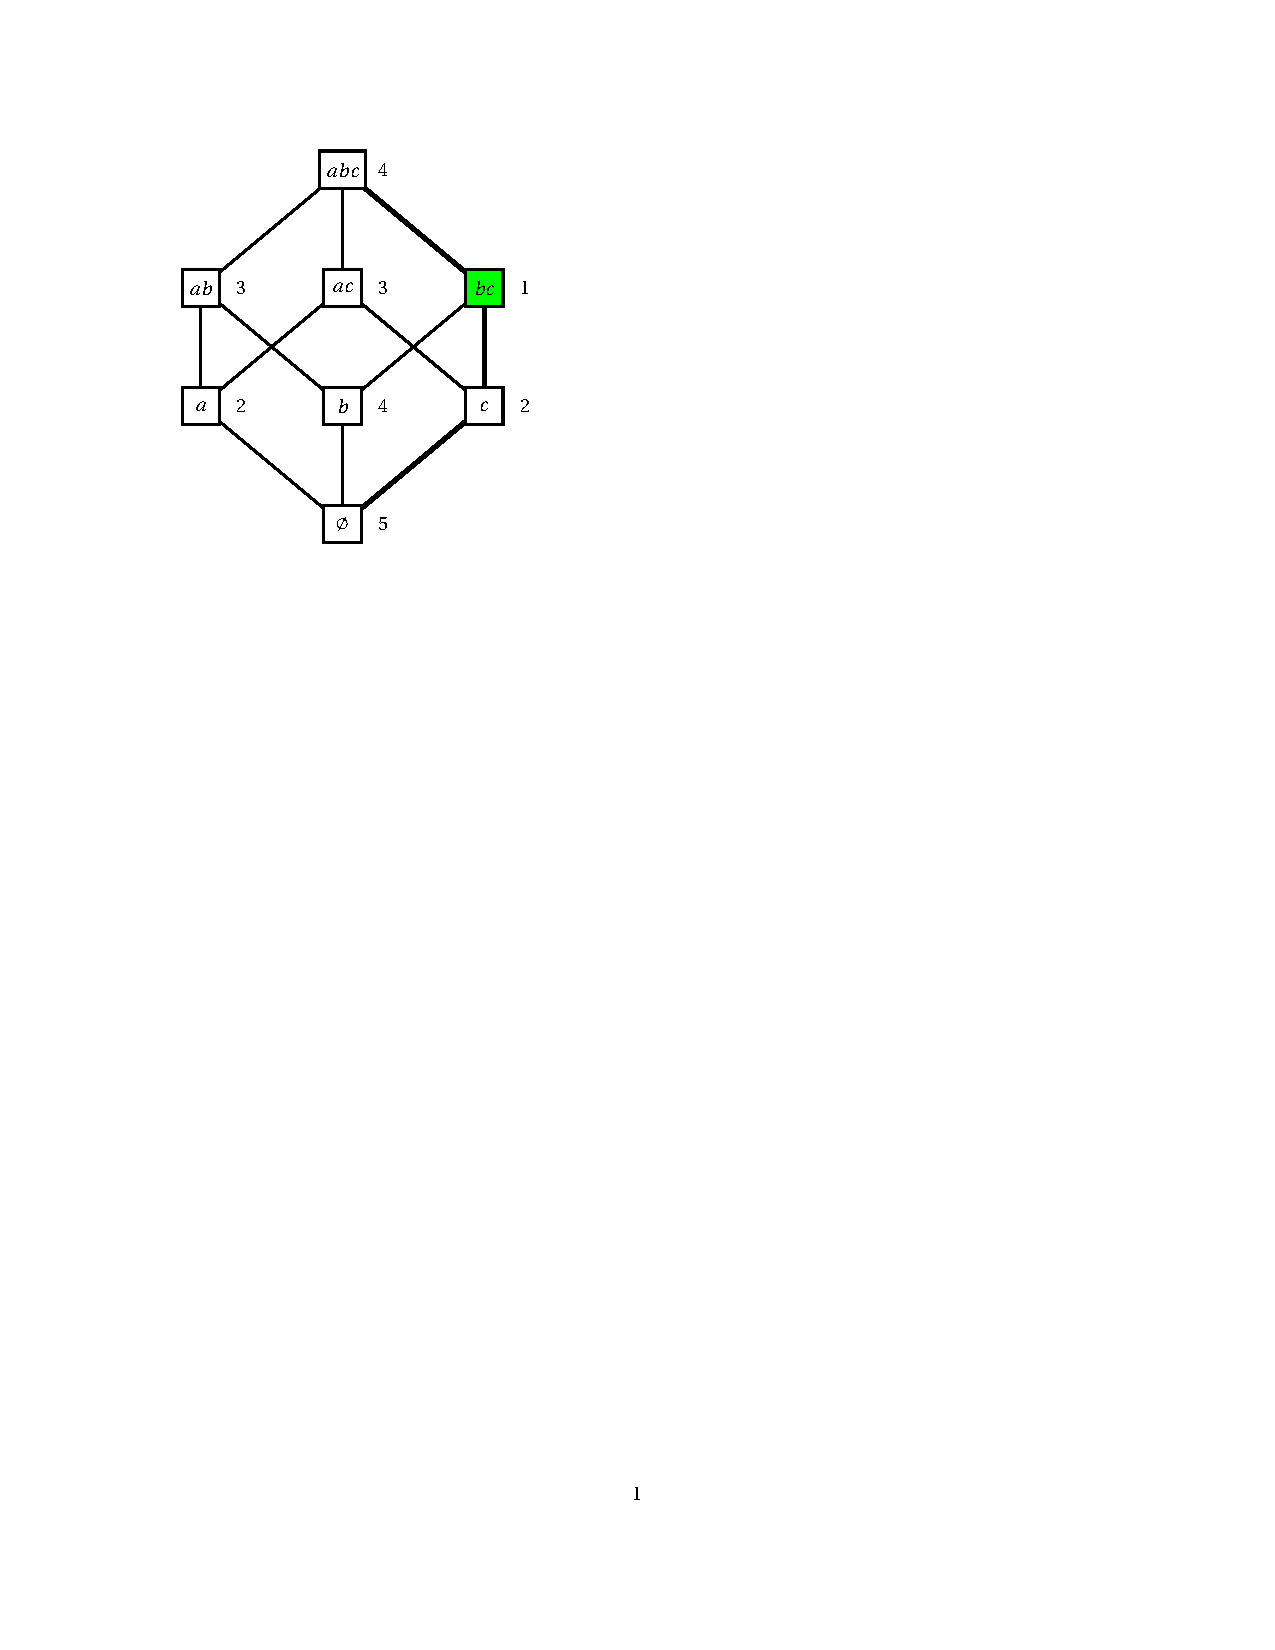
\includegraphics
        [trim=2cm 17.5cm 12.2cm 2cm,clip=true]{Boolean_lattice_3_A.pdf}}
        \label{fig:U-curve-example:A}
    }  
    &
    \subfigure[] {
        \scalebox{0.30}{
        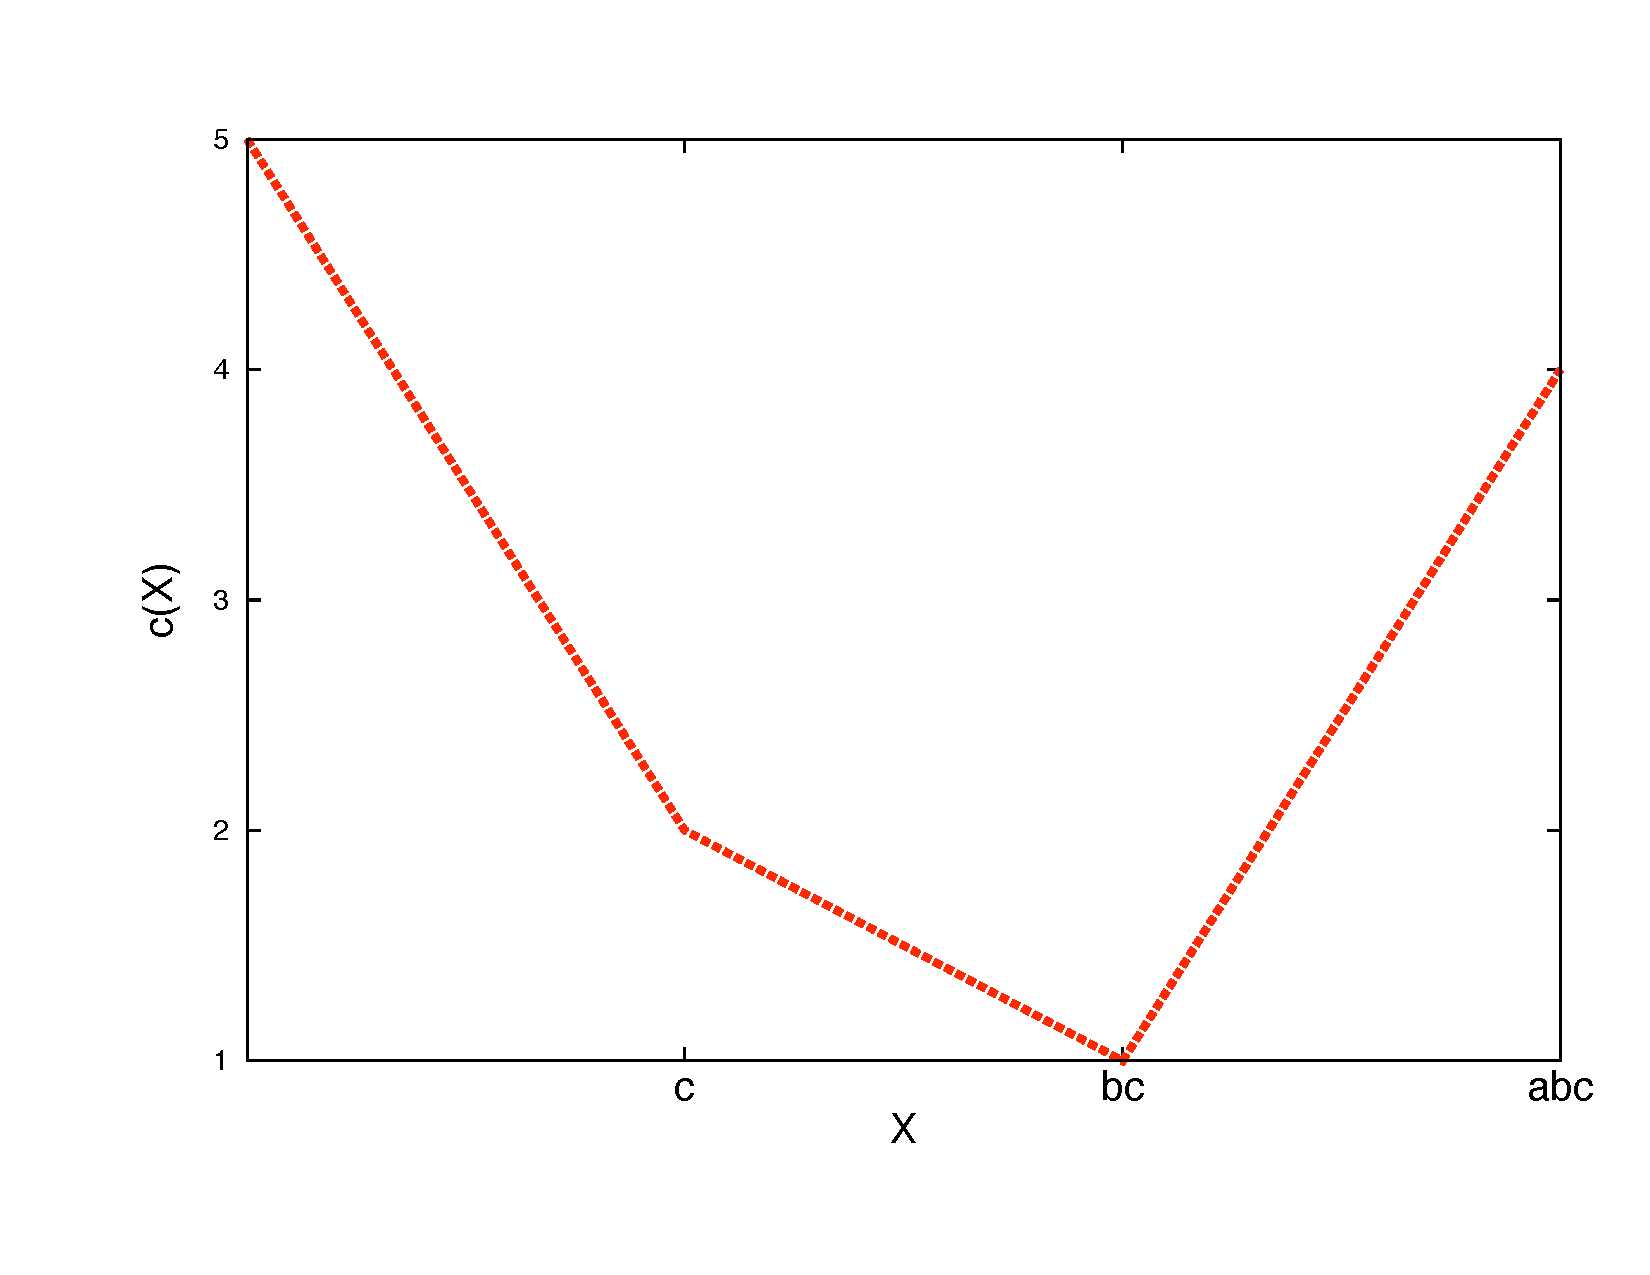
\includegraphics[clip=true]{exemplo1.pdf}} 
        \label{fig:U-curve-example:B} 
    }
\end{tabular}
\caption{um exemplo de instância do problema U-curve. 
Figura~\ref{fig:U-curve-example:A}: o diagrama de Hasse de um reticulado
Booleano de grau $3$ -- as cadeias do reticulado, cujos custos de seus
elementos são definidos através dos números ao lado dos nós, descrevem
curvas em U; a cadeia maximal $\{ \emptyset, c, bc, abc \}$ está
destacada em negrito. O elemento $bc$, destacado em verde, é mínimo na
cadeia (e também no reticulado Booleano). 
Figura~\ref{fig:U-curve-example:B}: o gráfico dos custos em função dos
elementos da cadeia maximal destacada em negrito, mostrando sua curva em
U. Figura extraída de Reis~\cite{msreis thesis}.} 
    \label{fig:U-curve} 
\end{figure}


% Levando-se em consideração tais limitações, existe a necessidade de
% novos algoritmos para atacar esse problema. Nesse sentido, foi 
% proposto o algoritmo Poset-Forest Search (PFS) (Reis, 2012, capítulo 
% 6.2 ~\cite{msreis thesis}). Uma versão preliminar foi implementada e
% testada, com resultados promissores; todavia, novos melhoramentos e
% testes são necessários para que o PFS se torne uma alternativa
% competitiva para resolver o problema de seleção de características.
\subsection{O algoritmo Poset-Forest Search}
O algoritmo {\tt PFS} é um algoritmo ótimo do tipo 
{\em branch-and-bound}. Esse algoritmo define duas florestas que são 
subgrafos do reticulado booleano que define o espaço de busca. Essas
florestas são compostas por árvores que são definidas por uma enumeração
arbitrária dos elementos do conjunto de característica. A ideia 
principal do algoritmo é, partindo de um raíz, percorrer um caminho 
dentro de uma árvore, fazendo podas no espaço de busca quando possível.

Uma versão preliminar desse algoritmo já foi implementada 
~\cite{msreis thesis} e mostrou resultados promissores, principalmente
quando analizado o número de nós do reticulado que são visitados. Apesar
disso, o algoritmo ainda pode ser estudado e apresenta características
que podem ser exploradas para melhorar seu desempenho. Para isso, 
podemos estudar o uso de ROBDDs para representar raízes das árvores na
floresta que representa o espaço de busca; paralelizar o percorrimento 
das árvores; e estudar modificações na dinâmica do algoritmo, que podem
se ajustar melhor as novas estruturas de dados, e também aproveitar
a estrutura do reticulado booleano.


\section{Objetivos}
Neste trabalho, propomos atingir os seguintes objetivos:

\begin{enumerate}
\item Utilização dos ROBDDs, implementados na iniciação científica
anterior, para representar as listas de raízes da floresta que 
representa o espaço de busca no algoritmo PFS.

\item Desenho de uma versão paralelizada do PFS, com maior
escalabilidade. Para este fim, paralelizaremos o percorrimento das
árvores nas florestas que representam o espaço de busca, com o programa
principal gerenciando a escolha das raízes (i.e., início de um 
percorrimento), guardando o mínimo corrente e centralizando a
atualização das podas.

\item Desenvolvimento de uma versão do PFS que funcione como algoritmo 
de aproximação para o problema U-curve, utilizando como critério de
aproximação da solução ótima o teorema da navalha de Ockham:\\
\smallskip
Dado um espaço de hipóteses H (i.e., espaço de busca), o número mínimo 
de amostras necessário para se obter uma solução que erra no máximo 
$\epsilon$ com $1 - \delta$ de probabilidade é expresso por:
\begin{equation}
\displaystyle  m(\delta,\epsilon) = 
    \frac{1}{\epsilon} log (\frac{|H|}{\delta}).
\end{equation}

\item Implementação e testes dos algoritmos propostos, para isso
empregando o arcabouço featsel.
\end{enumerate}


\section{Plano de trabalho}
A pesquisa se iniciará com o estudo do algoritmo {\tt PFS}. Esse 
algoritmo está atualmente implementado no arcabouço featsel, e será 
usado como base para os futuros algoritmos desse projeto. O próximo 
passo envolverá a construção de uma modificação do algoritmo {\tt PFS}
que utiliza a estrutura de dados ROBDD para guardar as raízes da 
floresta que representa o espaço de busca do problema.

Estudaremos em seguida a biblioteca OpenMP, escolhida para paralelização
do algoritmo. Após concluidos estudos da biblioteca, devemos analisar a
dinâmica do algoritmo {\tt PFS} e reescreve-la com as necessárias 
modificações para que partes do algoritmo possam ser executados em
paralelo. A principio, a paralelização do algoritmo se dará no 
percorrimento de caminhos das florestas do espaço de busca, que será 
atualizado em um espaço comum da memória a todas as linhas de execução.
Ao final dessa etapa, teremos um novo algoritmo, que será testado
e comparado com outros algoritmos do arcabouço featsel.

A próxima etapa do nosso trabalho será o estudo de algoritmos de 
aproximação e do modelo de aprendizado \textit{Probably Approximately
Correct} (PAC learning). Portanto, pretendemos construir uma variante do
algoritmo {\tt PFS} que deixa de buscar uma solução ótima para buscar
uma solução provavelmente aproximadamente correta. Utilizaremos como 
critério de aproximação a solução ótima do teorema da navalha de Ockham.

Após implementarmos o algoritmo de aproximação para o problema U-Curve
poderemos testar o seu desempenho com instâncias artificiais. Além 
disso, poderemos testar os algoritmos desenvolvidos durante o projeto
com instâncias reais do problema U-Curve. Os resultados obtidos, assim
como as descobertas feitas no processo de estudo e criação dos novos
algoritmos serão descritas em um artigo que será escrito como ultima 
atividade desse projeto.

\subsection{Cronograma}
Tabela listando atividades de janeiro a dezembro de 2017.

\begin{table}[!ht]
\caption{cronograma de atividades previstas neste projeto de
    Iniciação Científica. As descrições das atividades listadas seguem
    na seção a seguir.} 
\label{tab:cronograma}
\begin{center}
\smallskip
\begin{tabular}{l ccc ccc}
    \toprule
    \small Atividade/mês & \small Jan.17 & \small Fev.17 & \small Mar.17
                         & \small Abr.17 & \small Mai.17 & \small Jun.17
    \\ \hline

    \small Atividade 1   
    & \small {\bf x} & \small - & \small - & \small - & \small - \\

    \small Atividade 2   
    & \small {\bf x} & \small {\bf x} & \small - & \small - 
    & \small - \\

    \small Atividade 3   
    & \small - & \small {\bf x} & \small {\bf x} & \small - & \small -
    & \small - \\

    \small Atividade 4
    & \small - & \small - & \small {\bf x} & \small {\bf x} 
    & \small {\bf x} &  \small - \\

    \small Atividade 5   
    & \small - & \small - & \small - & \small - & \small {\bf x} 
    & \small {\bf x} \\

    \small Primeiro Relatório  
    & \small - & \small - & \small - & \small - & \small {\bf x} 
    & \small {\bf x} \\
    \bottomrule
    \toprule
    \small Atividade/mês & \small Jul.17 & \small Ago.17 & \small Set.17
                         & \small Out.17 & \small Nov.17 & \small Dez.17
    \\ \hline

    \small Atividade 6   
    & \small {\bf x} & \small {\bf x} & \small - & \small - & \small - 
    & \small - \\

    \small Atividade 7
    & \small - & \small {\bf x} & \small {\bf x} & \small{\bf x} 
    & \small - &  \small -\\

    \small Atividade 8  
    & \small - & \small - & \small - & \small {\bf x} & \small {\bf x} 
    & \small - \\

    \small Atividade 9
    & \small - & \small - & \small - & \small - & \small {\bf x} 
    & \small {\bf x}\\

    \small Segundo Relatório
    & \small - & \small - & \small - & \small - & \small {\bf x} 
    & \small {\bf x}\\
    \bottomrule
\end{tabular}
\end{center}
\end{table}

\subsection{Descrição de atividades}
\begin{itemize}
    \item{\bf Atividade 1.}
        Estudo do algoritmo {\tt PFS}.
    \item{\bf Atividade 2.}
        Implementação de uma variação do {\tt PFS} que usa ROBDDs como 
        estrutura de dados para representar início de caminhos.
    \item{\bf Atividade 3.}
        Estudo da biblioteca OpenMP, para paralelização do {\tt PFS}.
    \item{\bf Atividade 4.}
        Implementação de uma versão paralela do algoritmo {\tt PFS} com
        o uso de ROBDDs como estrutura de dados.
    \item{\bf Atividade 5.}
        Testes da primeira versão do {\tt PFS} paralelo com instâncias
        artificiais.
    \item{\bf Atividade 6.}
        Estudo do teorema da navalha de Ockham.
    \item{\bf Atividade 7.} 
        Implementação de uma variação do {\tt PFS} paralelo que se 
        comporte como um algoritmo de aproximação.
    \item{\bf Atividade 8.}
        Testes com instâncias artificiais do algoritmo de aproximação.
    \item{\bf Atividade 9.}
        Estudo comparativo entre os algoritmos produzidos, incluindo
        testes com instâncias reais.
\end{itemize}


% Arcabouço featsel, já contando com os acréscimos de classes de ROBDDs;
% Biblioteca OpenMP.
\section{Materiais e métodos}
Os algoritmos produzidos nesse trabalho serão implementados junto ao 
arcabouço featsel. Esse arcabouço foi implementado em C++ e conta com
diversas estruturas de dados que serão necessárias para implementar os
algoritmos sugeridos nesse trabalho. Além disso, o arcabouço featsel 
possui a estrutura de dados de ROBDDs, implementada em uma outra 
oportunidade de iniciação científica. 

O arcabouço featsel segue a licença \textit{GNU General Public License}
(GNU-GPL), o que nos permite utilizar o código do arcabouço para 
implementação dos novos algoritmos. Por utilizarmos o arcabouço como 
base, o código que será implementado nesse trabalho também seguirá a
licença GPL.

Também utilizaremos a especificação OpenMP junto ao compilador g++ para
compilar os códigos produzidos. A especificação OpenMP determina uma 
biblioteca que dá suporte ao programador, por meio de diretivas de 
compilação, ao determinar como um código pode ser executado em 
paralelo no processador.


% Benchmarking contra outros algoritmos de seleção de caracteríscas;
% Elaboração de paper para ser enviado para publicação ao final da IC
% proposta.
\section{Forma de Análise e de Divulgação dos Resultados}
Para analisar os resultados obtidos utilizaremos o próprio arcabouço
featsel, que já possui métodos que registram dados sobre a execução dos
algoritmos. As principais métricas a serem consideradas nos algoritmos
implementados serão tempo de execução e gasto de memória. As instâncias
utilizadas para geração desses dados serão tanto artificiais quanto 
reais, o que também nos oferecerá uma terceira métrica: a robustez dos
algoritmos quando violamos a suposição de que a função custo é 
decomponível em "curvas em u".

Após testarmos os algoritmos com instâncias reais e artificiais iremos
escrever um paper onde descreveremos os avanços que os novos algoritmos
trouxeram e quais características do problema U-Curve e de nossa solução
podem ser exploradas futuramente para elaboração de novas abordagens 
para resolver o problema.

\begin{thebibliography}{}
\addcontentsline{toc}{section}{Referências}
\bibitem{msreis thesis}
    Reis, Marcelo S. "Minimization of decomposable in U-shaped curves 
    functions defined on poset chains–algorithms and applications."
    PhD thesis, Institute of Mathematics and Statistics, University of
    São Paulo, Brazil, (2012).

\bibitem{ucsrobdd ic}
    %% como citar ic?

\end{thebibliography}
\end{document}
